%% Theory of Computing
%% File: v021a013.tex
%% Publication date: December 25, 2025
%% Authors: Joseph M. Landsberg and Mateusz Michalek
%
%
%
%

%
%

%
%
%
%
%
%
%
%
%
%
%
%
%
%

%

%
%
%
%
%
%
%
%
%
%
%
%
%
%
%
%
%
%
%
%
%
%

%

\documentclass{toc}

%
%
%
%
\tocdetails{%
  title = {Towards Finding Hay in a Haystack: Explicit Tensors of Border Rank Greater Than $2.02m$
in $\mathbb{C}^m\otimes \mathbb{C}^m\otimes \mathbb{C}^m$}, 
%
runningtitle = {Tensors of High Border Rank}, %
%
plaintexttitle = {Towards Finding Hay in a Haystack: Explicit Tensors of Border Rank Greater Than 2.02m in triple tensor product of m dimensional spaces}, %
%
  number_of_pages = {17}, 
  number_of_bibitems = {13},
  number_of_figures = {2},
  conference_version = {NONE}, %
    %
    %
%
%
%
  author = {Joseph Landsberg and Mateusz Micha{\l}ek},
    %
    %
    %
    %
    %
  authorlist = {Joseph Landsberg, Mateusz Micha{\l}ek},
    %
    %
    %
    %
    %
    %
    %
%
%
  %
  %
  %
  %
%
  acmclassification = {F.1.3},
    %
    %
  amsclassification = {15A69, 14L35, 68Q15},
    %
    %
  keywords = {matrix multiplication complexity, tensor rank, asymptotic rank, laser method},
    %
    %
    %
    %
    %
}   %

    %
    %
    %
    %
    %
    %
    %
    %
    %
    %
    %
    %
    %
    %
    %
    %
    %
    %
    %
    %
    %
    %
    %
    %
    %
    %
    %
    %
    %

%
%
\tocdetails{%
volume = 21,      %
number = 13,       %
year = 2025,
%
%
%
%
%
%
%
%
%
%
%
received = {May 11, 2021}, %
revised = {September 3, 2025},
published = {December 26, 2025},
%
%
%
doi = {10.4086/toc.2025.v021a013},
       %
}   %

%
%
%
%
%
 \usepackage{graphicx}   %

%
%
%
\newcommand{\aaa}{\mathbf{a}}
\newcommand{\bbb}{\mathbf{b}}
\newcommand{\ccc}{\mathbf{c}}
\newcommand{\vp}{\mathbf{V}\mathbf{P}}
\newcommand{\vnp}{\mathbf{V}\mathbf{N}\mathbf{P}}
\newcommand{\ot}{\otimes}
\newcommand{\ur}{\underline{\mathbf{R}}}
\newcommand{\BC}{\mathbb{C}}
\newcommand{\BZ}{\mathbb{Z}}
\DeclareMathOperator{\tlog}{log}
\newcommand{\mmm}{\mathbf m}\def\nnn{\mathbf n}
\newcommand{\Mn}{M_{\langle \nnn \rangle}}
\newcommand{\tmin}{\operatorname{min}}  %% ToC edit1 <-- no need for this: \min works
\newcommand\tsupp{{\rm supp}}
\newcommand\tmax{\operatorname{max}}    %% ToC edit1 <-- no need for this: \max works
\newcommand\tdim{\operatorname{dim}}    %% ToC edit1 <-- no need for this: \dim works
                   %% \min, \max, \dim are built-in LaTeX commands
\newcommand\PP{\mathbb P}
\newcommand\BT{\mathbb  T}
\newcommand\cA{{\mathcal A}}
\newcommand\cB{{\mathcal B}}
\newcommand\trank{\operatorname{rank}}
\newcommand\uR{\underline{\mathbf{R}}}
\newcommand\inv{{}^{-1}}
\newcommand{\Id}{\operatorname{Id}}

\usepackage{blkarray}
\usepackage{tikz}
\usetikzlibrary{arrows,shapes.geometric,positioning,decorations.markings,decorations.pathreplacing}
\definecolor{amethyst}{rgb}{0.6, 0.4, 0.8} 

\begin{document}

\begin{frontmatter}%

%
%
%

%
\title{Towards Finding Hay in a Haystack: Explicit Tensors of Border Rank Greater Than $2.02m$
in $\mathbb{C}^m\otimes \mathbb{C}^m\otimes \mathbb{C}^m$}  %

%
%

%
%
%
%
%
%

%
%
%
%
%
%
%
%
%
%
%
%


%
%
%
%

%

%
\author[michalek]{Mateusz Micha{\l}ek\thanks{Supported %
by the Deutsche Forschungsgemeinschaft — Projektnummer 467575307.}}
\author[landsberg]{Joseph Landsberg\thanks{Supported by NSF grants  AF-1814254 and AF-2203618.}}

%
%
%
%

%
%
%
%
%
%
%
%
\begin{abstract}
  We write down an explicit sequence of tensors in $\mathbb{C}^m\otimes \mathbb{C}^m\otimes \mathbb{C}^m$, for all $m$ sufficiently large, having border rank
  at least $2.02m$, overcoming a longstanding barrier. We obtain our lower bounds
via the border substitution method.
\end{abstract}

\iffalse %
%
%
%
%
%
%
%
%
%
%
%
%
%
%
%
%
%
%
%
%
%

\tocarxivcategory{cs.CC,math.AG}

\fi %

\end{frontmatter}

%
%
%
\section{Introduction}
A frequently occurring theme in algebraic complexity theory is the \emph{hay in a haystack}
problem (phrase due to %
Howard Karloff):
find an explicit object that behaves generically. For example Valiant's $\vp$ vs.~$\vnp$
problem is to find an explicit polynomial sequence that is difficult to compute.
We address this problem for three-way tensors. Here the state of the art is embarrassing.


Let $A,B,C$ be complex vector spaces %
of respective  %
dimensions $\aaa,\bbb,\ccc$. A tensor $T\in  A \ot B\ot C$ has \emph{rank one} if $T=a\ot b\ot c$ for some 
$a\in A$, $b\in B$, $c\in C$. The \emph{rank} of $T$, denoted $\mathbf R(T)$, is the 
smallest $r$ such that $T$ is a sum of $r$ rank one tensors.
 The \emph{border 
rank} of $T$, denoted $\ur(T)$, is the smallest $r$ such that $T$ is the limit of a 
sequence of rank $r$ tensors. 

If a tensor  $T\in \BC^m\ot \BC^m\ot \BC^m$ is chosen randomly with $m>3$, then with probability
one, it will have  rank and border rank $\lceil \frac{m^3}{3m-2}\rceil\sim \frac{m^2}3$~\cite{MR87f:15017} 
\footnote{The conclusion holds with almost any notion of %
randomness,  %
\eg, view the ambient $\BC^{m^3}$ as a vector space
with any measure that is absolutely continuous with respect to Lebesgue measure. Then the set of tensors for which the equality fails has measure zero.
If instead one takes the entries of $T$ from a finite subset of the integers with a uniform distribution, then the probability of
the equality failing goes to zero as the subset one draws from increases towards all of $\BZ$.}
.
 More precisely, the
set  of tensors with    border rank less than $\lceil \frac{m^3}{3m-2}\rceil$ is a proper subvariety and the
set of tensors with rank  not equal to  $\lceil \frac{m^3}{3m-2}\rceil$ is contained in a proper subvariety. 
Previous to this paper, there was no explicit sequence of tensors of
 border rank at least $2m$ known (and no explicit
sequence of
rank at least $3m$ known), although several known sequences come close to these.
In~\cite{MR3025382} they exhibit an explicit sequence of tensors satisfying
$\mathbf R(T_m)\geq 3m-O(\tlog_2(m))$
and in~\cite{MR3320240} a sequence of tensors of border rank at least $2m-2$ is presented,
although these tensors are only \lq\lq mathematician explicit\rq\rq\ and not
\lq\lq %
computer-scientist  %
explicit\rq\rq\ 
as some entries of the tensor are of the form $2^{2^m}$. We explain  the notion of
%
explicitness %
%
in \expref{Section}{subs:whatEX}.  %
The best border rank lower bound for
a %
%
computer-scientist-explicit  %
tensor to our knowledge is ironically the tensor $\Mn$ corresponding 
to matrix multiplication of $\nnn\times \nnn$
matrices where, setting $m=\nnn^2$,  $\ur(\Mn)\geq 2m-\lceil\frac 12 \tlog_2(m)\rceil-1$~\cite{MR3842382}. One of the central problems is that the typical way to prove that a tensor $T$ has high border rank is to determine a polynomial $P$ that vanishes on each tensor of border rank $r$ and prove that $P(T)\neq 0$. This shows that the border rank of $T$ is strictly greater than $r$. Still, in spite of many results  (see, \eg,  \cite{GO60survey} and references therein), there are no known polynomials on the space $\BC^m\ot \BC^m\ot \BC^m$ that vanish on tensors of border rank $2m$. For this reason the bound $2m$ remained unbroken until now. Here, instead of finding new polynomials vanishing on tensors of high rank, we combine several  methods: border substitution, Koszul flattenings
(which are polynomials),  combinatorics of normal forms, degenerations as well as explicit computational techniques. In this paper
we deal exclusively with border rank.


\begin{definition} \label{explicitdef}
 A sequence of objects (\eg, numbers, graphs, tensors, typically each represented as a finite sequence of integers), indexed by integers, %
 is \emph{explicit}  if the $n$-th object may be computed in time polynomial in $n$. 
\end{definition}

We remark that there are more restrictive definitions of
what it means for a sequence to be explicit but the experts we asked viewed the above one as acceptable.



Thus, a 
 sequence $T_m\in \BC^m\ot \BC^m\ot \BC^m$ of tensors is explicit if the 
 entries of $T_m$  may be computed in time polynomial   in $m$. This is equivalent to saying  that all of $T_m$ may be computed in polynomial time in $m$. 

  We show:

\begin{theorem} \label{mainthm}
For each  $k$,    define the $\lceil \frac{3(2k+1)^2}{4}\rceil$-dimensional
family of tensors $T_k=T_k(p_{ij})\in \BC^{2k+1}\ot\BC^{2k+1}\ot\BC^{2k+1}=: A\ot B\ot C$ %
as follows:
\begin{equation}\label{Tk}
T_k=\sum_{i=-k}^k \sum_{j=\max(0,-i)}^{\min(2k-i,2k)}p_{i j} a_i\ot b_j\ot c_{i+j}\,,
\end{equation}
where $A\simeq B\simeq C\simeq \BC^{2k+1}$ and $(a_{-k},\dots, a_k),(b_{0},\dots, b_{2k}),(c_{0},\dots, c_{2k})$
are %
bases of the vector spaces
$A,B,C$,
respectively.  %

Then for all 
$$0<\epsilon<\frac 1{42}, {\rm \  and   \ }  k\geq
\frac{7 (52274 - 151635 \epsilon + 14616 \epsilon^2 + 5292 \epsilon^3)}{(1 - 42 \epsilon)^3 }\,,
$$
we describe  an explicit assignment of the $p_{ij}$ 
in the sense of \expref{Definition}{explicitdef}, so that

$$\ur(T_k)\geq (2+\epsilon)(2k+1)=(2+\epsilon)m\,.
$$

\end{theorem}

In particular,  when 
$\epsilon=.001$ we need $k\geq 414797$, %
%
 and when
 $\epsilon=.02$ we need
$k\geq 84162677$.

Viewing $T_k$ as a matrix of linear forms, \eg, $T(A^*)$, the matrix is zero in the upper right and lower left corners,
\eg, when $k=2$,
$$
T_2(A^*)=\begin{pmatrix}*&*&*&0&0\\  *&*&*&*&0\\ *&*&*&*&*\\  0&*&*&*&*\\   0&0&*&*&*\end{pmatrix}\,.
$$

The explicit assignment is as follows: for $|i|>\frac 37k$,  list the $p_{ij}$ in some order and assign them  
distinct  prime numbers as in \expref{Lemma}{expla}. For $|i|\leq \frac 37k$,   assign them periodically as in \expref{Lemma}{explb}. More precisely, 
set    $K=\lceil \frac{78}{1-42\epsilon}\rceil$. Then  the value of $p_{ij}$ depends only on $i \text{ mod } 4K$ and $j \text{ mod } 4K$. For $0\leq i,j<4K$
the values %
%
%
 of $p_{ij}$
are determined in such a way that 
%
%
%
 distinct values are never coordinates of 
%
a solution to any of the explicit nonzero polynomials that we derive in \expref{Lemma}{neardiagcase}. 


If $k$ is smaller, we can still get border rank bounds of twice the dimension or greater. For example:

\begin{theorem}\label{thm:explicit}
Let $T_6$ be assigned the values $p_{ij}=2^i+3^j-7ij$.
Then $\ur(T_6)\geq 26=2m$.
\end{theorem}

\subsection*{Acknowledgements}
We thank Markus Bl\"aser,  Michael Forbes and Josh Grochow for explaining various
definitions of explicitness to us, and the anonymous referees for useful comments.
%

\section{Background}
\begin{definition} Let $T\in A\ot B\ot C$ be a tensor and let $A^*_f\subset A^*$ be a linear subspace.
The \emph{restriction} of $T$ to $A_f^*$, denoted $T|_{A_f^*\ot B^*\ot C^*}=:T|_{A^*_f}$ is
obtained by identifying $T$ with a linear map $A^*\rightarrow B\otimes C$ and restricting the domain to the subspace $A_f^*$.  
\end{definition}
A tensor $T\in A\ot B\ot C$ is \emph{$A$-concise} if the induced map $A^*\rightarrow B\ot C$ is injective. Intuitively,   $T$ cannot be realized as a tensor in some  $\BC^{\aaa-1}\ot B\ot C$. 

The \emph{border substitution method} of~\cite{MR3633766} begins with the observation that, for each fixed $f<\aaa$ and $A$-concise tensor $T$,
\begin{equation}\label{submeth}
\ur(T)\geq \tmin_{A^*_f\subset A^*}\left(\aaa-f+\ur(T|_{A^*_f\ot B^*\ot C^*})\right)
\end{equation}
where the min is over all subspaces $A^*_f$ of $A^*$ of  dimension $f$.   
As stated, this is nearly useless as it is not practical to test all $f$-dimensional subspaces of $A^*$.
However, when a tensor has symmetry, the normal form lemma \cite[Lem. 3.1]{MR3633766} allows one
to restrict the search to a smaller subset. In particular, when it is invariant under a torus,
\ie, a continuous
abelian diagonalizable subgroup, it is sufficient to test the $A^*_f$ that are invariant under the action of the torus.
As observed by Strassen (and is well known among algebraic geometers), torus invariant objects
can be studied via combinatorics. In our situation, the relevant property is as follows:

For a tensor $T=\sum_{ijk}t^{ijk} a_i\ot b_j\ot c_k$ given in bases, the \emph{support} of $T$
is $\tsupp(T):=\{ (ijk)\mid t^{ijk}\neq 0\}$.

\begin{definition}[\cite{MR1089800}]   %
A tensor $T\in A\ot B\ot C$ is \emph{tight} 
%
%
%
if there exist bases of $A,B,C$  and  
injective functions $\tau_A : [\aaa] \to \BZ$, $\tau_B : [\bbb] \to \BZ$ and $\tau_C : [\ccc] \to \BZ$ such that
for all $(i,j,k) \in \tsupp(T)$, $\tau_A(i) + \tau_B(j) + \tau_C(k)=0$. (See~\cite{MR4204580}  for details.)
 Call such a basis a \emph{tight basis}.
\end{definition}

Given a tight basis, %
%
the tensor $T$ is invariant with respect to the $\BC\backslash\{ 0\}$-action
where $t\in \BC\backslash\{ 0\}$ acts on
%
%
%
%
%
the $i$-th, $j$-th, and $k$-th
basis vector of $A$, $B$, and~$C$ by multiplication by  $t^{\tau_A(i)}$
$t^{\tau_B(j)}$, and $t^{\tau_C(k)}$, respectively.


The \expeqref{tensor}{Tk}  %
is $A$-concise (for the given assignment of %
the $p_{ij}$  %
and tight with $\tau_A(i)=i$, $\tau_B(j)=j$, $\tau_C(k)=k$.

The border substitution method and normal form lemma of~\cite{MR3633766} imply:
\begin{proposition}\label{tightbapolarok}
Let $T\in A\ot B\ot C$ be tight,  $A$-concise, and expressed in a tight basis. Then among the filtrations $A_1^*\subset \cdots \subset A_{\aaa-1}^*\subset A^*$
of $A^*$,  \ie, among nested sequences of subspaces where $\tdim(A_f^*)=f$, 
where each $A^*_f$ is spanned by tight basis elements, there is at least one such that
$$
\ur(T)\geq \tmax_q(q+\ur(T(q)))\,,
$$
where $T(q):=T|_{A_{\aaa-q}^*\ot B^*\ot C^*}$.
\end{proposition}
For convenience of the reader, we give a self-contained proof:

\begin{proof} 
By induction on $\dim A^*$ it is enough to prove that we may choose $A_{\aaa-1}^*$ as in the proposition.
Fix $f:=\aaa-1$. For any $g\in GL(A)$,
if we replace $T$ by $gT$, and $A_f^*$ by $gA_f^*$  in \expeqref{Eq.}{submeth} 
the inequality still holds.
The Borel fixed point theorem (see, \eg, \cite[\S 21.2]{MR0396773}) says that a connected
solvable group acting on a complete variety $X$ has a fixed point in $X$. In our case the 
connected solvable
group is the torus $\BT=\BC\backslash\{0\}$ and $X$ is the $\BT$-orbit closure
of some $A^*_{f,0}\in G(f,A^*)=\PP(A)$ achieving the minimum in \expeqref{Eq.}{submeth}.
Since $gT=T$ for all $g\in \BT$, the right hand side of \expeqref{Eq.}{submeth} is
unchanged. Finally  the $\BT$-fixed points are exactly the $f$-planes spanned
by basis vectors.  
\end{proof}

Thus tight tensors are a natural class of tensors where the border substitution method may
be
effectively implemented because there are only a finite number of filtrations to check.
The family $T_k$ of %
\expref{Theorem}{mainthm} is tight.

If $T$ is tight, then any tensor with the same support as $T$ in a tight basis is also tight. In particular, it
is natural to study tight tensors in families indexed by the support. In this context, 
it was shown in~\cite{MR4204580} that the largest possible  support  
for a tight tensor is given by the   \expeqref{family}{Tk},  
which  is a $\lceil \frac 34 m^2\rceil$-dimensional
family, where $m=2k+1$. That is, the \expeqref{family}{Tk}
is the largest such
that \expref{Proposition}{tightbapolarok} may be applied to.

The idea of the proof of \expref{Theorem}{mainthm} is as follows: think of a game where we are trying to
prove a lower bound and an adversary is trying to prevent it by zeroing out basis vectors
of $T_k$ in a way that lowers the border rank  of the degenerated tensor as much as possible. We show that, no matter
what strategy the adversary chooses, there is a $q$ where we obtain the desired lower bound
using the Koszul flattenings described in
%
\expref{Section}{kossect}  %
by further degenerating the already degenerated
tensor to make the lower bound estimate from the Koszul flattenings transparent.  
After describing   Koszul
flattenings, in %
\expref{Section}{mainpf}  %
we group the adversary's possible strategies into three types, and show
that  for each
strategy we can choose a $q$ and a further degeneration to obtain our bound.

\section{Explicit tensors}\label{subs:whatEX}

The following  two types of sequences of tensors are explicit in the sense of 
\expref{Definition}{explicitdef}.

\begin{lemma}\label{expla} Let $T_m\in \BC^m\ot \BC^m\ot \BC^m$ be a sequence of tensors whose only nonzero entries
are as in \expeqref{tensor}{Tk}.   %
If the entries of $T_m$ are the first distinct $m^2$ prime numbers, then $T_m$ is explicit.
\end{lemma}
\begin{proof}
Let $\pi(x)$ be the number of prime numbers smaller or equal than $x$.  By~\cite{rosser1962approximate}
we know that $\frac{x}{\log x}<\pi(x)$ for $x\geq 17$. Hence, running the sieve method on first $m^3$ numbers, 
we may find the  first $m^2$ prime numbers in polynomial time. 
\end{proof}

The following is obvious but we record it for future use:

\begin{lemma}\label{explb}Let $T_m\in \BC^m\ot \BC^m\ot \BC^m$ be a sequence of tensors whose only nonzero entries
are as in \expeqref{tensor}{Tk}.  %
If the entries of $T_m$ 
are taken from a fixed library $\{ c_{a,b}\}_{0\leq a< \cA, 0\leq b< \cB}$ of
integers periodically, so $p_{ij}=c_{(i\text{ mod }\cA),(j\text{ mod }\cB)}$), then the sequence $T_m$ is explicit.
\end{lemma}
  
The tensors in our  sequence will be a sum of tensors of the types from \expref{Lemmas}{expla} \expref{and}{explb}, and thus
also explicit.

\section{Koszul  flattenings and border rank lower bounds}\label{kossect}
We first review Koszul flattenings. 
 We then  apply Koszul flattenings to a projection of the tensor $T_6$ and two general types of tensors, each of which
arises as a degeneration  of $T_{k,q}:=T_k|_{A^*_{2k+1-q}\ot B^*\ot C^*}$.

\subsection{Koszul flattenings}\label{subsec: generalized flattenings}
Fix an integer $p<\frac 12 \tdim A$.
Fix bases $\{a_i\}$, $\{b_j\}$, $\{ c_k\}$ of   $A,B,C$. Let  
$T = \sum_{ijk} t^{ijk} a_i \otimes b_j \otimes c_k \in A \otimes B \otimes C$. Consider the linear map
\begin{align*}
T_A^{\wedge p}: \Lambda^p A \ot B^* &\to \Lambda^{p+1}A\ot C \\
X\ot \beta & \mapsto \sum_{ijk}t^{ijk}\beta(b_j)(a_i\wedge X) \ot c_k.
\end{align*}
Then  \cite[Proposition 4.1.1]{MR3081636} states 
\begin{equation}\label{kozinq}
\ur(T)\geq \frac{\trank(T_{A}^{\wedge p})}{\binom {\tdim(A)-1}p}\,.
\end{equation}

Let ${A'}^*\subset A^*$ be a subspace. Write $\phi : A \to A/ 
({A'}^*)^\perp=:A'$ for the projection onto the quotient.
Here $({A'}^*)^\perp\subset A$ is the annihilator of ${A'}^*\subset A^*$.
The corresponding Koszul 
flattening map gives a lower bound for $\uR(\phi(T))$, which, by linearity, is 
a lower bound for $\uR(T)$.

One often  takes a subspace ${A'}^*\subseteq A^*$ of dimension $2p+1$ in the restriction of
  $T$, so the denominator $\binom{\dim(A)-1}{p}$ is 
replaced by $\binom{2p}{p}$ in \expeqref{Eq.}{kozinq}.  

The $p=1$ case is a generalization of  Strassen's equations~\cite{Strassen505}, and
for tensors in 
$\BC^m\ot \BC^m\ot \BC^m$ it  can at best prove border rank lower bounds of $\frac 32m$.
 The larger the $p$ one takes, Koszul flattenings become  closer to potentially being
 able to prove a border rank lower bound
 of $2m$. However, the equations become more difficult to implement.
We  utilize the $p=2$ case, which 
can at best prove border rank lower bounds of $\frac 53m$. This case can be reduced
to lower bounding a matrix whose entries are at worst cubic in the $p_{ij}$ of
\expeqref{tensor}{Tk}.  %
Thus,  before using Koszul flattenings, 
 we will need to use the border substitution method to kill off  at least a 
$(\frac 13+\epsilon)m$-dimensional space.
In our case  we will  kill off  a space of dimension  
$\sim\frac{1}{2}m$ because our Koszul flattening matrices will not be of maximal rank.

\newcommand{\qz}{\hspace{-0.05em}}    %
%
    
Let $T\in \BC^5\ot \BC^n\ot \BC^n$ and write
$T=a_1\ot X_1+\cdots + a_5\ot X_5$.
Order the bases of $\bigwedge^2\BC^5$, $a_i\wedge a_{i'}$, with  
%
$ii'=12,\qz 13,\qz 14,\qz 15,\qz 23,\qz 24,\qz 25,\qz 34,\qz 35,\qz 45$
and of $\bigwedge^3\BC^5$ as
$234,\qz 235,\qz 245,\qz 345,\qz 123,\qz 124,\qz 125,\qz 134,\qz 135,\qz 145$.
Then the $10n\times 10n$ Koszul flattening matrix takes
the block form
\begin{equation}
    \label{big10}T_{A}^{\wedge 2}=
\begin{blockarray}{ccccccccccc}
12&13&14&15&23&24&25&34&35&45&\\
\begin{block}{(cccccccccc)c}
0&0&0&0& X_4&-X_3&0&X_2&0&0 &234\\
0&0&0&0& X_5&0&-X_3&0&X_2&0&235 \\
0&0&0&0& 0&X_5&-X_4&0&0&X_2&245 \\
0&0&0&0& 0&0&0&X_5&-X_4&X_3&345 
\\
X_3&-X_2 &0& 0& X_1&0&0&0&0&0&123 \\
X_4&0 &-X_2& 0& 0&X_1&0&0&0&0&124 \\
X_5&0 &0&-X_2&        0&0&X_1&0&0&0&125 \\
0&X_4 &-X_3&0&  0&0&0&X_1&0&0&134 \\
0&X_5 &0&-X_3&        0&0&0&0&X_1&0&135 \\
0&0 &X_5&-X_4&        0&0&0&0&0&X_1&145 \\
\end{block}
\end{blockarray}\,.
\end{equation}

If $X_1$ is invertible then %
the rank of the \expeqref{matrix}{big10} equals
$6n$ plus the rank of the block $4n\times 4n$ matrix with block entries
\begin{equation}\label{p2matrix}
\begin{pmatrix}
X_3X_1^{-1} X_4-X_4X_1^{-1}X_3&X_4X_1^{-1} X_2-X_2X_1^{-1}X_4&X_2X_1^{-1} X_3-X_3X_1^{-1}X_2&
0\\
X_3X_1^{-1} X_5-X_5X_1^{-1}X_3&X_5X_1^{-1} X_2-X_2X_1^{-1}X_5&0&X_2X_1^{-1} X_3-X_3X_1^{-1}X_2
\\
X_4X_1^{-1} X_5-X_5X_1^{-1}X_4&0&X_5X_1^{-1} X_2-X_2X_1^{-1}X_5&
X_2X_1^{-1} X_4-X_4X_1^{-1}X_2\\
0&X_4X_1^{-1} X_5-X_5X_1^{-1}X_4&X_5X_1^{-1} X_3-X_3X_1^{-1}X_5&
X_3X_1^{-1} X_4-X_4X_1^{-1}X_3\end{pmatrix}\,.
\end{equation}

To see this use the basic identity, for a block matrix with 
$Z$ square and invertible: 
$$
\begin{pmatrix}
0&X\\ Y&Z\end{pmatrix}
=
\begin{pmatrix} 
\Id & XZ\inv \\ 0 &\Id\end{pmatrix}
\begin{pmatrix}
-XZ\inv Y & 0 \\ 0&Z\end{pmatrix} 
\begin{pmatrix} \Id & 0\\
Z\inv Y & \Id
\end{pmatrix}\,.
$$

\newcommand{\qw}{\hspace{-0.45em}}    %
%
In what follows it will be more convenient to permute the blocks of
the \expeqref{matrix}{p2matrix}  %
and multiply rows and columns by $(-1)$, so that the matrix becomes block skew-symmetric:
\begin{equation}\label{p2matrixb}
\begin{pmatrix}
0&\qw 
-X_2X_1^{-1} X_3+X_3X_1^{-1}X_2 
&\qw  X_4X_1^{-1} X_2-X_2X_1^{-1}X_4&\qw 
-X_3X_1^{-1} X_4+X_4X_1^{-1}X_3
\\
X_2X_1^{-1} X_3-X_3X_1^{-1}X_2
&\qw 0&\qw -X_5X_1^{-1} X_2+X_2X_1^{-1}X_5&\qw 
X_3X_1^{-1} X_5-X_5X_1^{-1}X_3
\\
X_2X_1^{-1} X_4-X_4X_1^{-1}X_2
&\qw X_5X_1^{-1} X_2-X_2X_1^{-1}X_5
&\qw 0&\qw X_4X_1^{-1} X_5-X_5X_1^{-1}X_4
\\
X_3X_1^{-1} X_4-X_4X_1^{-1}X_3
&\qw X_5X_1^{-1} X_3-X_3X_1^{-1}X_5
&\qw -X_4X_1^{-1} X_5+X_5X_1^{-1}X_4&\qw 
0
\end{pmatrix}\,.
\end{equation}

We record the above observation. %

\begin{proposition}\label{blockred} Let $T=a_1\ot X_1+\cdots + a_5\ot X_5\in \BC^5\ot \BC^n\ot \BC^n$ and let $X_1$ be
of   rank $n$.
If   the rank of the $4n\times 4n$ \expeqref{block matrix}{p2matrix}
is at least 
$R$, then $\trank(T_{A}^{\wedge 2})\geq R+6n$.
\end{proposition}

\subsection{Proof of \expref{Theorem}{thm:explicit}}
We first project $T_6$ to $\BC^9\otimes \BC^{13}\otimes \BC^{13}$ by considering all possible coordinate projections. By \expref{Proposition}{tightbapolarok} for one of the projections the border rank drops at least by four.
In the algorithm
used  in %
\expref{Section}{codesect},  %
all possible $\binom{13}{4}$ projections are considered. 

Next, in each case we consider a general projection to $\BC^5\otimes \BC^{13}\otimes \BC^{13}$. We note that we do not have to prove that the chosen projection is general, as it is enough to find one projection. 
Finally we apply $p=2$ Koszul flattenings described in \expref{Section}{subsec: generalized flattenings}. The algorithm, implemented in Macaulay~2~\cite{M2}, checks
that  %
the rank of
the \expeqref{matrix}{big10}  %
is always at least $127$.  Thus:  %
\[ \ur (T_6)\geq \lceil \frac{127}{6}\rceil+4=22+4=26\,. \qedhere \]
\qed

\subsection{Koszul flattenings applied to  a tensor with $T(A^*)$ supported on the diagonal
  and four  
%
  shifted diagonals close to the diagonal}

Recall that a Zariski open subset of a vector space is the complement of the zero set of a finite
collection of polynomials on the space. In particular, given a fixed nonempty open subset, a random
element of a vector space will lie in the subset with probability one.
\begin{definition}
%
  A 
%
shifted   
  diagonal of a matrix $(m_{ij})$
 at distance $y$ below %
 (or above) %
 the diagonal
 is the set of those entries where $i - j = y$ %
 ($j-i=y$, resp.).
 A diagonal corresponds to the case $i = j$.  We call a matrix a
%
shifted-diagonal if it is
 supported on a 
 %
shifted 
 diagonal.
 \end{definition}

 \begin{lemma}\label{neardiagcase}
Let $T=a_1\ot X_1+\cdots + a_5\ot X_5\in \BC^5\ot \BC^n\ot \BC^n$ be a tensor such that
$X_1$ is diagonal with nonzero entries on the diagonal, 
 $X_2,X_3$ are 
%
 shifted-diagonal matrices supported on 
%
shifted 
 diagonals
at distances  $x_2< x_3$
above the main diagonal and $X_4,X_5$ are 
%
 shifted-diagonal matrices  supported on 
%
shifted 
  diagonals $x_4<x_5$
below the main diagonal, and assume $x_s<C$ for $s=2,\ldots,5$ for some constant $C$.

Fixing one such $T$  as above,    the $p=2$ Koszul flattening matrix drops rank by at most
$16C$ on a Zariski open subset of tensors with the same  shape as $T$. 
In particular, for most  tensors $T$ of that shape, 
$\ur(T)\geq \frac 53 n-\frac 83 C$. 
\end{lemma}

\begin{proof}
As $X_1$ is invertible, the second Koszul flattening 
has a kernel of dimension equal to the dimension of the kernel  of
the \expeqref{matrix}{p2matrix}.  %

Write $M_{ts}:=X_tX_1^{-1} X_s-X_sX_1^{-1}X_t$, $t<s$, for the six  distinct  size $n\times n$
block matrices appearing in
the \expeqref{matrix}{p2matrix} %
(here $M_{st}=-M_{ts}$). 
The $M_{ts}$   are 
%
 shifted-diagonal
matrices. Explicitly, $M_{23}$ is supported on 
%
 shifted diagonal $x_2+x_3$,
$M_{24}$ is supported on 
%
 shifted diagonal $x_2-x_4$, $M_{25}$ is supported on   %
 shifted  
 diagonal $x_2-x_5$,
$M_{34}$ is supported on 
%
 shifted 
 diagonal $x_3-x_4$, $M_{35}$ is supported on 
 %
 shifted 
 diagonal $x_3-x_5$,
$M_{45}$ is supported on 
%
 shifted
 diagonal $-(x_4+x_5)$,
where negative indices mean the 
%
shifted 
diagonal is below the main diagonal. We note that some of the entries on these 
%
 shifted
 diagonals may be equal to zero.

Permuting the basis vectors, one obtains a  block diagonal matrix, where the blocks are
of size $4\times 4$, namely, using cyclic notation, we group columns
$x_5+j$, $x_4+j$, $-x_3+j$, $-x_2+j$
and rows $j-x_2-x_3+x_4,j-x_2-x_3+x_5,j-x_2+x_4+x_5,j-x_3+x_4+x_5$, and there are $n$ such blocks, as in \expref{Figure}{fig:4x4}.
Call the resulting $4\times 4$  blocks $N^j$, $1\leq j\leq n$.

It remains to show
that  %
almost all matrices $N^j$ have full rank. We note that each of the matrices $M_{ts}$ has at most $4C$ entries on the distinguished 
%
shifted 
diagonal that are not a binomial in the entries of %
the $X_i$.  %
These non-binomial entries appear only if one of the column or row indices of $M_{ts}$ is either smaller than $2C$ or greater than $n-2C$. We focus on 
%
the $N^j$   %
%
contained in the other rows and columns, \ie, $2C<j<n-2C$. A direct computation shows that the determinant of each such $N^j$ is, after clearing denominators, an explicit nonzero polynomial $P^j$ in the entries of the matrices $X_i$. We note that in the given range of indices the polynomials $P^j$ are evaluations of one polynomial, but in different sets of variables.

Hence, whenever the evaluations of the $n-4C$  polynomials $P^j$ are nonzero
the bounds on ranks given in \expref{Lemma}{neardiagcase} hold.  
\end{proof}
\begin{figure}[ht]\begin{center}

%
 \begin{tikzpicture}[line width = 0.5 mm, scale=0.70]  %

        %
        %
        %
        
        \draw[red] (4.2,16) -- (8,12.2);
        
        \draw[green!60!black!100] (8, 15.6) -- (11.6, 12);
        
        \draw[blue] (12, 15.4) -- (15.4, 12);
        
        \draw[red] (0.2,12) -- (4,8.2);
        
        \draw[green!60!black!100] (0, 7.6) -- (3.6, 4);
        
        \draw[blue] (0, 3.4) -- (3.4, 0);
        
        \draw[orange] (8, 11.8)--(11.8,8);
        
        \draw[orange] (4, 7.8)--(7.8,4);
        
        \draw[amethyst] (12, 11.6) -- (15.6,8);
        
        \draw[amethyst] (4, 3.6) -- (7.6,0);
        
        \draw[yellow!60!green!100] (12,7) -- (15,4);
        
        \draw[yellow!60!green!100] (8,3) -- (11,0);

        %
        %
        %
        %
        \draw[dashed, yshift = 1.1] (2.2,0)--(2.2,16) node[midway, yshift = 4.7cm, xshift = -0.5cm]{\huge 0};
        
        \draw[dashed, yshift = 1.1] (6.4,0)--(6.4,16) node[midway, yshift = 1.9cm, xshift = -0.5cm]{\huge 0};
        
        \draw[dashed, yshift = 2.15] (9.8,0)--(9.8,16) node[midway, yshift = -1.2cm, xshift = 0.55cm]{\huge 0};
        
        \draw[dashed, yshift = 2.6] (13.6,0)--(13.6,16) node[midway, yshift = -4.25cm, xshift = 0.55cm]{\huge 0};
        
        \draw[dashed, xshift = 1.1] (0,13.8)--(16,13.8);
        
        \draw[dashed, xshift = 0.6] (0,10)--(16,10);
        
        \draw[dashed, xshift = 1.35] (0,5.4)--(16,5.4);
        \draw[dashed, xshift = 1.5] (0,1.2)--(16,1.2);

        %
        %
        %
        
        \draw[black,fill=white, line width = 0.3 mm] (2.2,1.2) circle (1ex);
        
        \draw[black,fill=white, line width = 0.3 mm] (6.4,1.2) circle (1ex);
        
        \draw[black,fill=white, line width = 0.3 mm] (9.8,1.2) circle (1ex);
        
        \draw[black,fill=white, line width = 0.3 mm] (2.2,5.4) circle (1ex);
        
        \draw[black,fill=white, line width = 0.3 mm] (6.4,5.4) circle (1ex);
        
        \draw[black,fill=white, line width = 0.3 mm] (13.6,5.4) circle (1ex);
        
        \draw[black,fill=white, line width = 0.3 mm] (2.2,10) circle (1ex);
        
        \draw[black,fill=white, line width = 0.3 mm] (9.8,10) circle (1ex);
        
        \draw[black,fill=white, line width = 0.3 mm] (13.6,10) circle (1ex);
        
        \draw[black,fill=white, line width = 0.3 mm] (6.4,13.8) circle (1ex);
        
        \draw[black,fill=white, line width = 0.3 mm] (9.8,13.8) circle (1ex);
        
        \draw[black,fill=white, line width = 0.3 mm] (13.6,13.8) circle (1ex);

        %
        
        \draw[step=4,black] (0,0) grid (16,16);
        
        %
        %
        %
        
        \draw[decorate,decoration={brace,amplitude=5pt,raise=0.5ex}]
        (0,16) -- (2.2,16) node[midway,yshift=0.5cm]{$i+x_5$};
        
        \draw[decorate,decoration=
        {brace,amplitude=5pt,raise=0.5ex}]
        (4,16) -- (6.4,16) node[midway,yshift=0.5cm]{$i+x_4$};
        
        \draw[decorate,decoration=
        {brace,amplitude=5pt,raise=0.5ex}]
        (8,16) -- (9.8,16) node[midway,yshift=0.5cm]{$i-x_3$};
        
        \draw[decorate,decoration=
        {brace,amplitude=5pt,raise=0.5ex}]
        (12,16) -- (13.6,16) node[midway,yshift=0.5cm]{$i-x_2$};
        
         \draw[decorate,decoration=
        {brace,amplitude=5pt,raise=0.5ex,mirror}]
        (0,16) -- (0,13.75) node[midway,xshift=-1.5cm]{$i-x_2-x_3+x_4\text{\ \quad}$};
         %
         
        \draw[decorate,decoration=
        {brace,amplitude=5pt,raise=0.5ex,mirror}]
        (0,12) -- (0,10) node[midway,xshift=-1.5cm]{$i-x_2-x_3+x_5\text{\ \quad}$};
        %
        
        \draw[decorate,decoration=
        {brace,amplitude=5pt,raise=0.5ex,mirror}]
        (0,8) -- (0,5.4) node[midway,xshift=-1.5cm]{$i-x_2+x_4+x_5\text{\ \quad}$} ;
        %
        
        \draw[decorate,decoration=
        {brace,amplitude=5pt,raise=0.5ex,mirror}]
        (0,4) -- (0,1.2) node[midway,xshift=-1.5cm]{$i-x_3+x_4+x_5\text{\ \quad}$};
        %

        %
        %
        %
        
        \draw[decorate,decoration=
        {brace,amplitude=1pt,raise=0.5ex,mirror}]
        (4,16) -- (4.2,16) node[midway,rotate=270,xshift= 0.8cm,yshift=0.12cm]{$x_3+x_2$};

        \draw[decorate,decoration=
        {brace,amplitude=1pt,raise=0.5ex,mirror}]
        (0,12) -- (0.2,12) node[midway,rotate=270,xshift= 0.8cm,yshift=0.12cm]{$x_3+x_2$};

        %
        %
        %
        
        \draw[decorate,decoration=
        {brace,amplitude=2pt,raise=0.5ex}]
        (8,16) -- (8,15.6) node[midway,xshift=0.8cm, yshift=-0.05cm]{$x_4-x_2$};
        \draw[decorate,decoration=
        {brace,amplitude=3pt,raise=0.5ex}]
        (12,16) -- (12,15.4) node[midway,xshift=0.8cm, yshift=-0.02cm]{$x_4-x_3$};
        \draw[decorate,decoration=
        {brace,amplitude=1pt,raise=0.5ex}]
        (8,12) -- (8,11.8) node[midway,xshift=0.8cm, yshift=-0.07cm]{$x_5-x_2$};
        \draw[decorate,decoration=
        {brace,amplitude=2pt,raise=0.5ex}]
        (12,12) -- (12,11.6) node[midway,xshift=0.8cm,yshift=-0.05cm]{$x_5-x_3$};
        \draw[decorate,decoration=
        {brace,amplitude=5pt,raise=0.5ex}]
        (12,8) -- (12,7) node[midway,xshift=0.9cm]{$x_4+x_5$};
        
        %
        %
        %

        %
        
        \draw[decorate,decoration=
        {brace,amplitude=2pt,raise=0.5ex}]
        (0,8) -- (0,7.6) node[midway,xshift=0.8cm, yshift=-0.05cm]{$x_4-x_2$};
        \draw[decorate,decoration=
        {brace,amplitude=1pt,raise=0.5ex}]
        (4,8) -- (4,7.8) node[midway,xshift=0.8cm, yshift=-0.08cm]{$x_5-x_2$};
        \draw[decorate,decoration=
        {brace,amplitude=3pt,raise=0.5ex}]
        (0,4) -- (0,3.4) node[midway,xshift=0.8cm]{$x_4-x_3$};
        \draw[decorate,decoration=
        {brace,amplitude=2pt,raise=0.5ex}]
        (4,4) -- (4,3.6) node[midway,xshift=0.8cm,yshift=-0.05cm]{$x_5-x_3$};
        \draw[decorate,decoration=
        {brace,amplitude=5pt,raise=0.5ex}]
        (8,4) -- (8,3) node[midway,xshift=0.9cm]{$x_4+x_5$};
    \end{tikzpicture}
  
\caption{\expeqref{Matrix}{p2matrixb} for a tensor as in \expref{Lemma}{neardiagcase}  after permuting basis vectors as in the proof. The $i$-th $4\times 4$ block $N^i$ has entries corresponding to the intersection of the dashed lines}\label{fig:4x4}
\end{center}
\end{figure}
\begin{corollary}\label{cor:subTkclosediag}
Let $T$ be a tensor as in \expref{Lemma}{neardiagcase}
that is such a subtensor\footnote{%
%
A \emph{subtensor} is %
a tensor defined by the same formula as $T_k$, where we only sum over subsets of indices} of the tensor $T_k$ that all  $X_i$ correspond to 
%
shifted 
diagonals of $T$ of distance at most $\frac{3}{7}k$ to the main
%
diagonal\footnote{\Ie, we only %
take $a_i$ such that $|i|\leq \frac{3}{7}k$ in \expeqref{Equation}{Tk}}. Then the assertion of the \expref{Lemma}{neardiagcase} holds.
\end{corollary}
\begin{proof}
We keep the notation of \expref{Lemma}{neardiagcase} and its proof.

We note that each $P^j$, irrespective of the choice of $T$ and $j$, depends only on variables corresponding to entries that are contained in a $4C\times 4C\times 4C$ subtensor of $T_k$  made of consecutive indices, \ie,~$(T_{k})_{i,j,l}$, where $i\in \{N_1+1,N_1+C\}$, $j\in \{N_2+1,N_2+4C\}$ and $l\in \{N_3+1,N_3+C\}$ for some integers $N_1,N_2,N_3$. As $C$ is a fixed constant and
the  %
$P^j$ are explicit polynomials, the non-vanishing can be achieved by filling
one $4C\times 4C\times 4C$ cube with numbers 
%
that do not form coordinates of any root of 
%
%
%
 any of the $P^j$   %
%
%
and then assigning the values of the tensor periodically as in \expref{Lemma}{explb}.
\end{proof}

%

\subsection{Koszul flattenings applied to  a tensor supported on $5$ 
%
shifted
diagonals not equal to the diagonal}


\begin{lemma}\label{primecase}
Let $T\in \BC^5\ot \BC^{n}\ot \BC^{n}$ be a tensor supported on 
three 
%
shifted 
diagonals at distances $y_3<y_4<y_5$ below the diagonal and two 
%
shifted 
diagonals
at distances $y_1>y_2$ above the diagonal such that $y_1-y_2<y_3$ and $y_1+y_5<n$.
Assume the entries of $T$ are distinct primes.
Then
$$
\ur(T)\geq n+y_1-\frac 23 y_2\,.
$$
\end{lemma}
\begin{proof}
Consider the second Koszul flattening matrix of $T$ given in \expeqref{Eq.}{big10}. The bound of $\ur(T)$ will follow by estimating the rank of this matrix.
 
Consider,  in each of the last six blocks,
the last $n-y_1$ columns. We obtain $6n-6y_1$ independent columns  due to the matrix $X_1$ in
\expeqref{Eq.}{big10}. 

We now restrict our attention to columns that are still in last six blocks, but
just consider the  first $y_1$ columns in each block. We focus on the upper four horizontal blocks, obtaining a $4n\times 6y_1$ matrix, as in \expref{Figure}{fig:4x6}. Note that in order for the lines in each block to have width $y_1$ we need  $y_1+y_5<n$. 
We claim that the rank of this matrix is at least $4y_1+2(y_1-y_2)$.

In this matrix the second, third and sixth vertical blocks give independent columns, due to the matrices that are $y_3$ below the diagonal (blue in \expref{Figure}{fig:4x6}). We claim that the $y_1$ columns in the first vertical block are also independent of  them. For contradiction suppose there is a linear relation involving $i$-th column in the first block. The $(i+y_4)$ entry of the first block of this column may only be canceled using the $(i+y_4-y_3)$ column in the second block. Then the contribution in the third block may only be canceled by the $(i+y_5-y_3)$ column in the third vertical block. Now the entries in the second horizontal block cancel if and only if a binomial cubic equation on the entries is satisfied. This is not possible, as the entries are distinct primes. 

So far we obtain the lower bound on the rank of matrix in \expref{Figure}{fig:4x6} equal to $4y_1$. By adding
the  last $(y_1-y_2)$ columns of fourth and fifth block, which are independent as $y_1-y_2<y_3$, we may find $2(y_1-y_2)$ more independent columns. 


We now focus on the first four vertical blocks in
the \expeqref{matrix}{big10}.  %
Among those,
the first four horizontal blocks are zero, thus we restrict to the last six. We further restrict to the rows that are zero in last six vertical blocks. We obtain a $6\times 4$ block matrix, which is similar to reflection of the matrix in \expref{Figure}{fig:4x6}. We lower bound  the rank of this matrix in 
the same way as before.

In total we obtain that the rank of
the \expeqref{matrix}{big10} is at least  %
$$6(n-y_1)+2(4y_1+2(y_1-y_2))=6n+2(3y_1-2y_2).$$
This   translates to the bound on the border rank as in the statement of the lemma.
\end{proof}
\begin{figure}[ht]\begin{center}
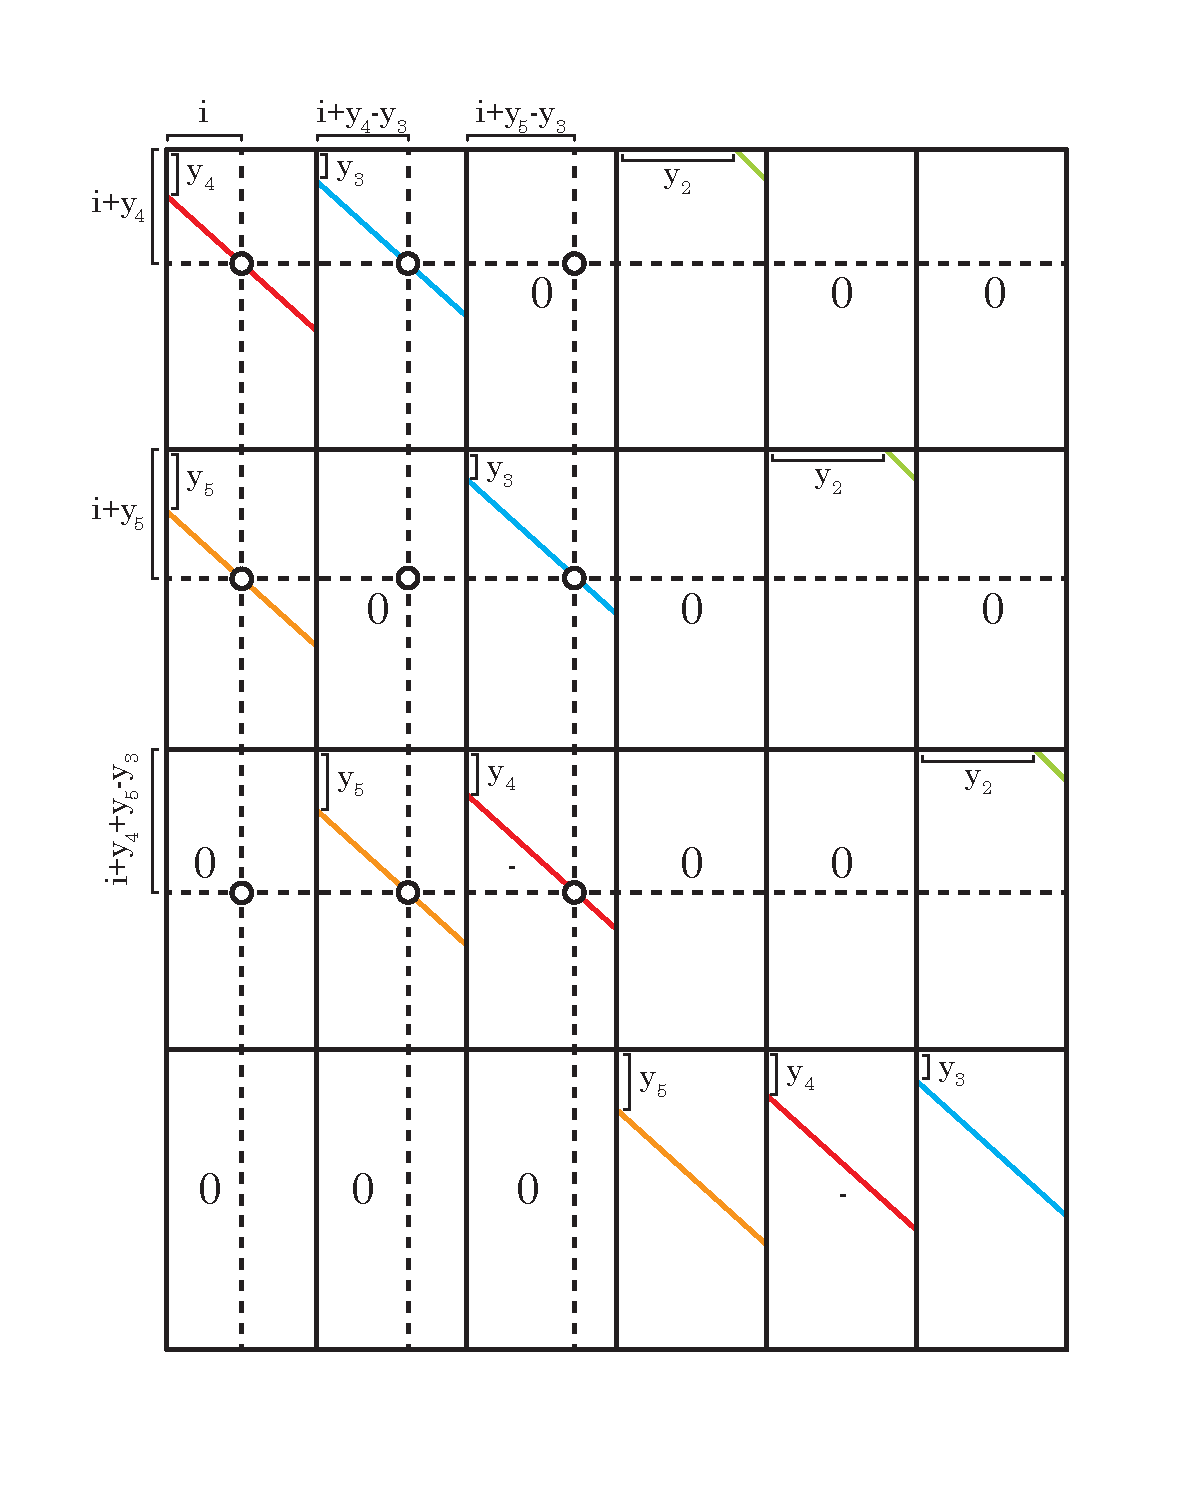
\includegraphics[scale=0.5]{fig4x6}
\caption{The size $4n\times 6y_1$ submatrix of the  $4n\times 6n$ matrix.}
\label{fig:4x6}
\end{center}
\end{figure}

\section{Proof of \expref{Theorem}{mainthm}}\label{mainpf}
%
 
We need to 
find explicit $p_{ij}$ for the \expeqref{sequence}{Tk}
and to lower bound the border ranks of   $T_{k,q}=T_k|_{A_{2k+1-q}^*\ot
  B^*\ot C^*}$
  as in \expref{Proposition}{tightbapolarok} for all
sufficiently large $k$ and some
useful $q=q(k)$.
We first determine $q$. (Imagine our  choice of $q$ being based on  the strategy of our opponent.)




Let $I_q$ denote the index set kept  to obtain $T_{k,q}$,  so $|I_q|=2k+1-q$.
Write  $I_q=I_{-}\sqcup I_0\sqcup I_{+}$ for the negative, zero, and positive indices appearing in $I_q$. Note that   the sets $I_{-}, I_0, I_{+}$ depend on $q$ and if we want to stress this dependence we  write $I_{-}(q)$. Fix a large constant $K$   to be determined later.
In what follows $0<\epsilon<\frac 1{42}$\,.

{\bf Setup}: Let $T_{k,q}$ be a sequence of restrictions as above.  Let  $q$ be the largest index   such that in each of $I_-(q),I_+(q)$ there exist
either 
\begin{enumerate}
\item Three indices with absolute value at least $\frac k2$, or
\item Five indices with absolute value smaller than $\frac k2$ such that the
absolute value of the difference
of the smallest and largest one is at most $K$.
\end{enumerate}

Without loss of generality we may assume that   both conditions fail for $I_-(q+1)$. 

\begin{lemma}\label{lem:belowsmall} Let $T_{k,q}$ and $q$ be as in the setup.
Then  $|I_-|\leq \frac{2k}{K}+7$ and hence
$q\geq k-(\frac{2k}{K}+7)$.
\end{lemma}
\begin{proof}
Partition  the negative indices $\{-k,\ldots, -1\}$  into groups  as follows:
\begin{enumerate}
\item $\{-k,\ldots, -\lceil \frac k2\rceil\}$
\item $\lfloor (k/2)/K\rfloor$ groups 
\begin{align*}\{-\lceil \frac k2\rceil+1,\ldots, -\lceil \frac k2\rceil+K\},\ 
 \{-\lceil \frac k2\rceil+K+1,\ldots, -\lceil \frac k2\rceil+2K\} \ 
 ,\ldots, \\ 
 \{-\lceil \frac k2\rceil+(\lceil \frac k2\rceil -1)K+1,\ldots, -\lceil \frac k2\rceil+ \lfloor (k/2)/K\rfloor K\}
 \end{align*}
\item $\{-\lceil \frac k2\rceil+ \lfloor (k/2)/K\rfloor K+1,\ldots, -1\}$
\end{enumerate}
 As the conditions fail for $q+1$ we can have at most four indices in $I_-(q+1)$ in each of the groups in $(2)$ or in group $(3)$ giving at most:
\[4\frac{k}{2K}+4=\frac{2k}{K}+4\]
indices in groups $(2)$ and $(3)$ for $I_-(q+1)$. In the group $(1)$ we can have at most $2$ indices. 
The cardinality of $I_-(q)$ and $I_-(q+1)$ may differ at most by one. The bounds follow.
\end{proof}
We now group the possible distributions of indices in the %
sets $I_q$  %
into three
cases and show that in each case we may obtain the desired lower bound.
Note that the size of $q$ we utilize to obtain the lower bound will depend on
  how the indices are removed.
 
\begin{lemma}\label{claim:no5large} Let $T_{k,q}$ and $q$ be as in the setup and $K \geq \frac{78}{1 - 42 \epsilon}$.
If  
\begin{equation}
    \label{claimhyp}
|I_{+}\cap[0,\frac{3}{7}k]|> \frac{4}{K}\frac{3}{7}k+4\ \ {\rm or}\ \ |I_{-}\cap[-\frac{3}{7}k,0]|> \frac{4}{K}\frac{3}{7}k+4\,,
\end{equation}
then 
for all $k>\frac{210K+21K\epsilon-168+56K^2}{K-78-42K\epsilon}$\,, one has
$\ur(T_k)\geq (2+\epsilon)(2k+1)$\,.
\end{lemma}
\begin{proof} 
Recall that $m=2k+1$. 
Suppose  $|I_{+}\cap[0,\frac{3}{7}k]|> \frac{4}{K}\frac{3}{7}k+4$. We partition $\{0,\dots,\lfloor\frac{3}{7}k\rfloor\}$ into at most $\lfloor\frac{3k}{7K}\rfloor+1$ subsets of consecutive indices of cardinality at most $K$. By the pigeonhole principle
we may find five indices $i_1<\dots<i_5\leq \frac{3}{7}k$ in $I_{+}$ with $i_5-i_1\leq K$. If we choose
the  smallest possible such indices, then $q\geq k-(\frac{2k}{K}+7)+ i_3-\frac 4K i_3-4$.

Restrict $T$ to the subspace of $B^*\ot C^*$ where  $i_3$ becomes the diagonal.
By \expref{Lemma}{neardiagcase} and \expref{Corollary}{cor:subTkclosediag}, with $n=m-i_3$ and $C=K$,  
we have $\ur(T_{k,q})\geq \frac 53(m-i_3)-\frac 83K$.
Thus $\ur(T_k)\geq \frac{13}{3}k-\frac{2}{3}i_3-\frac{4}{K}i_3-(\frac{2k}{K}+\frac{28}{3})-\frac 83K$. As $i_3\leq \frac{3}{7}k-2$ we 
need
$$
\left(\frac {13}3-\frac 23\frac 37\right)k+(-2-\frac{4\cdot 3}7)\frac{k}K +\frac{8}K - \frac 83K-8\geq (2+\epsilon)(2k+1),
$$
\ie,
$$
k\geq \frac{210K+21K\epsilon-168+56K^2}{K-78-42K\epsilon}.
$$

Now instead  assume $|I_{+}\cap[0,\frac{3}{7}k]|\leq \frac{4}{K}\frac{3}{7}k+4$ 
and thus  $q\geq k-(\frac{2k}{K}+7)+\frac{3(K-4)}{7K}k-4$. Using this, we may conclude   in the
case $|I_{-}\cap[-\frac{3}{7}k,0]|> \frac{4}{K}\frac{3}{7}k+4$ by the same reasoning as above with an even better bound.  
\end{proof}
In light of \expref{Lemmas}{lem:belowsmall} \expref{and}{claim:no5large}, we may henceforth
assume \expeqref{Eq.}{claimhyp} %
fails  to hold so 
\begin{equation}\label{qbnd}
q\geq
k-\left(\frac{2k}{K}+7\right)+\frac 37k-\frac{12k}{7K}-4=\frac{10}{7}k-\frac{26k}{7K}-11\,.
\end{equation}

\begin{lemma} \label{lem:far}  Let $T_{k,q}$ and $q$ be as in the setup and assume
additionally that \expeqref{Eq.}{qbnd} holds.
If  $I_{-}$ has three indices with absolute value greater than $\frac{k}{2}$,
then
$\ur(T_k)\geq (2+\epsilon)(2k+1)$ when
$ K\geq \frac{39}{1-21\epsilon}$ 
and
$ 
k\geq \frac{(13+\epsilon)21K}{2(K-39-21K\epsilon)}
$\,.
\end{lemma}
\begin{proof}
Let $y_3,y_4,y_5$ be   three indices in $I_{-}$ with absolute value greater
than $\frac{k}{2}$\,. Let 
$y_1$ and $y_2$ be %
the largest and smallest index in $I_{+}\setminus [0, \frac{k}{2} ]$,
respectively,  %
which exist by point $(1)$ of the %
setup.  %
Thus, we may add
$\frac k2-(y_1-y_2)-1$ to \expeqref{Eq.}{qbnd}. 
By \expref{Lemma}{primecase} with $n=2k+1$ we obtain:
\begin{align*}\ur(T_k)&\geq \ur(T_{k,q})+q\\
&\geq 
2k+1+y_1-\frac{2}{3}y_2+\frac{10}{7}k-\frac{26k}{7K}-11+\frac{k}{2}-(y_1-y_2)-1\\
&\geq \frac{86}{21}k-\frac{26}{7}\frac kK-11,
\end{align*}
where to obtain the last  line we used that $y_2\geq \frac{k}{2}$.

This bound will be greater than $(2+\epsilon)(2k+1)$ when
$$
K\geq 
\frac{39}{1-21\epsilon}
$$
and
$$
k\geq\frac{(13+\epsilon)21K}{2(K-39-21K\epsilon)}
$$
%
%
concluding the proof of 
\expref{Lemma}{lem:far}. %
\end{proof}

\begin{lemma} \label{lem:near}
 Let $T_{k,q}$ and $q$ be as in the setup and assume
additionally that \expeqref{Eq.}{qbnd} holds.
If  $I_{-}$ has five  indices with absolute value smaller than $\frac{k}{2}$
such that the difference of the smallest and largest is at most $K$, 
then
$\ur(T)\geq (2+\epsilon)(2k+1)$ when
$
K\geq \frac{78}{1-42\epsilon}
$
and
$
k\geq \max(\frac{21(12+ \epsilon)K}{K-42\epsilon K-78},\frac{210K+21K\epsilon-168+56K^2}{K-78-42K\epsilon}).
$
\end{lemma}
\begin{proof}
Suppose these five indices have absolute value less or equal to $\frac{3}{7}k$. Then we conclude exactly as in the first part of the proof of \expref{Lemma}{claim:no5large}. Thus, we assume all indices are greater then $\frac{3}{7}k-K$.

We proceed as in \expref{Lemma}{lem:far}. First assume there exist two indices in $I_{+}\setminus [0,\frac{4}{7}k+K]$. Fix $y_2$ and $y_1$ to be, respectively, %
the smallest and largest index in $I_{+}\setminus [0,\frac{4}{7}k+K]$,
so we may add $\frac{3}7k-K-(y_1-y_2)$ to \expeqref{Eq.}{qbnd}.

We obtain:
\begin{align*}
\ur(T_k)&\geq \ur(T_{k,q})+q\\
&\geq \left(2k+1+y_1-\frac 23 y_2\right)+ \frac{10}{7}k-\frac{26k}{7K}-11+\frac 37 k-K-(y_1-y_2)\\
&\geq (4+\frac 1{21})k-\frac{26}{7}\frac kK -10-\frac{2K}{3},
\end{align*}
where in the last line we used that $y_2\geq \frac 47k+K$.
This is at least $(2+\epsilon)m$ when
$$
K\geq \frac{78}{1-42\epsilon}
$$
and
$$
k\geq \frac{21(12+ \epsilon+\frac{2K}{3})K}{K-42\epsilon K-78}
$$
and we conclude in this case.

If there are no two indices in $I_{+}\setminus [0,\frac{4}{7}k+K]$, then by point (1) in the setup we must have two indices in $I_{+}\cap [\frac{1}{2}k, \frac{4}{7}k+K]$. Let $y_2$ and $y_1$ to be, respectively, %
the smallest and largest in this set.
We may add $\frac{1}{2}k-1-(y_1-y_2)$ to \expeqref{Eq.}{qbnd}. Note that $y_1-y_2<\frac{3}{7}k-K$. Proceeding as above obtain an even stronger lower estimate on border rank.
\end{proof}
\begin{proof}[Proof of \expref{Theorem}{mainthm}]
One of the cases in \expref{Lemmas}{claim:no5large},
%
\ref{lem:far}, \expref{and}{lem:near} must hold, 
which proves the theorem for $k$ large enough.

In order for
the  %
assumptions of all lemmas to hold,  we need $K\geq \frac{78}{1-42\epsilon}$ and
$k\geq \frac{21(12+ \epsilon+\frac{2K}{3})K}{K-42\epsilon K-78}$
 and $k\geq \frac{210K+21K\epsilon-168+56K^2}{K-78-42K\epsilon}$.
As $K\geq 78$, the last lower bound on $k$ is more restrictive.  
Taking the estimate $K=\frac{78}{1-42\epsilon}+1$ 
 it holds when
 \[k\geq \frac{7 (52274 - 151635 \epsilon + 14616 \epsilon^2 + 5292 \epsilon^3)}{(1 - 42 \epsilon)^3 }\,.  \qedhere \] 
 \end{proof}

 \section{Code for the proof of \expref{Theorem}{thm:explicit}}\label{codesect}
\begin{verbatim}
S=QQ[w_0..w_4];
rs=res ideal basis(1,S);
kosz=rs.dd_3;
R=QQ[a_(-6)..a_6,b_(-6)..b_6,c_(-6)..c_6,w_0..w_4] 
T6:=0
for i from -6 to 6 do
(
 for j from max(-6,-i-6) to min(6,-i+6) do
  ( 
   T6=T6+(2^i+3^j-7*i*j)*a_i*b_j*c_(-i-j)
  ); 
)
by=matrix{{b_(-6)..b_6}}; cz=matrix{{c_(-6)..c_6}};
L=subsets(-6..6,4); zle={};
for m in L do (
subp={};
 for mm from -6 to 6 do(
  if (not member(mm,m)) then(
   subp=subp|{a_mm=>(sum for i from 0 to 4 list (random(0,R)*w_i))};
  );
 );
 l= rank diff(cz,diff(transpose by,diff(sub(kosz,R),sub(T6,subp))));
if (l<127) then zle=zle|{m};
)
#zle
\end{verbatim}

\bibliographystyle{tocplain}   %

%
%
%
%
\bibliography{bibstrings,v021a013,bibtail}

%
%
%
%
%
\begin{tocauthors}
%
\begin{tocinfo}[landsberg] %
Joseph Landsberg\\
 Owen Professor of Mathematics\\
 Department of Mathematics\\  
 Texas A\&M  University\\
 College Station, Texas, USA\\
 jml@math.tamu.edu \\   %
 \url{https://people.tamu.edu/~jml/}      %
\end{tocinfo}
%
\begin{tocinfo}[michalek]  %
  Mateusz Micha{\l}ek\\
  Professor in real algebraic geometry\\
  University of Konstanz\\
  Konstanz, Germany\\
  mateusz.michalek\tocat{}uni-konstanz\tocdot{}de \\
  %
    \href{https://www.mathematik.uni-konstanz.de/working-group-real-geometry-and-algebra/prof-dr-mateusz-michalek/}{https://www.mathematik.uni-konstanz.de/ \newline working-group-real-geometry-and-algebra/prof-dr-mateusz-michalek/}
\end{tocinfo}
\end{tocauthors}

%
%
%
%
%
%
%
%
%
%
%
%
%
%
%
%
%
%
%
%
\begin{tocaboutauthors}
\begin{tocabout}[landsberg]  %
  \textsc{Joseph (JM) Landsberg} %
works on  geometric problems originating in complexity theory. He
obtained his \phd\ in 1990 from Duke University under the direction of Robert Bryant
on minimal submanifolds and a generalization of calibrations. 
His past research  was   at the interface of algebraic geometry, differential geometry 
and representation theory.
He is an Owen Professor of Mathematics at Texas A\&M University. 
Landsberg   has directed 
fifteen  \phd\ theses, is the author of five books:
\begin{itemize}  %
%
\item \emph{Quantum Computation and Quantum Information: A Mathematical Perspective},
%
AMS %
  %
  %
  (2024)
   %
   %
   [\href{https://bookstore.ams.org/view?ProductCode=GSM/243}{AMS Bookstore}] %
\item \emph{Tensors:  Asymptotic Geometry and  Developments 2016-2018}, AMS 
%
(2019)  %
  %
[\href{https://bookstore.ams.org/view?ProductCode=CBMS/132}{AMS Bookstore}] %
\item \emph{Geometry and Complexity Theory},
  Cambridge U. Press (2017)  %
%
  [\href{https://www.cambridge.org/core/books/geometry-and-complexity-theory/15E3ABA3FF14E1054574663F60250D80}{CUP}]  %
\item \emph{Tensors: Geometry and Applications}, AMS (2012)  %
%
[\href{https://bookstore.ams.org/view?ProductCode=GSM/128}{AMS Bookstore}]  %
\item \emph{Cartan for Beginners} (co-author Thomas A. Ivey), 
  AMS (2003), 2nd edition (2016)   %
  %
[\href{https://bookstore.ams.org/view?ProductCode=GSM/175}{AMS Bookstore}]  %
\end{itemize}
and has published over 100 research articles.
Fall 2025 he %
co-organized  %
the semester ``Complexity and Linear algebra'' %
at the Simons Institute for the Theory of Computing, UC Berkeley.
At the same time he   also served as a   UC Berkeley Chancellor's Professor.
Landsberg was first exposed to the beauty of geometry in college while taking
a calculus course for Physics majors being taught by Joe Harris,
and first exposed to complexity by Peter B\"urgisser, who
offered him a bottle of champagne if he could solve a question about
$2\times 2$ matrices. 
\end{tocabout}
%
\begin{tocabout}[michalek]  %
\textsc{Mateusz Micha{\l}ek} is an algebraic geometer by training and a combinatorist at heart. He earned his \phd\ in 2012 from the Polish Academy of Sciences, supervised by Jaros{\l}aw Wi\'sniewski, and Universit\'e Joseph Fourier, supervised by Laurent Manivel. He held postdoc positions at Berkeley, FU Berlin, MPI Bonn, Oberwolfach, IMPAN Warsaw, the University of Barcelona, and RIMS Kyoto. After a few great years leading a research group at MPI MiS Leipzig, he settled at the University of Konstanz-—where he claims to be equally inspired by theorems, the lake, and the Alps (in no particular order).
\end{tocabout}
\end{tocaboutauthors}

%

%
  
%
 
%

\end{document}

